\documentclass{article}

%Margins
\usepackage[margin=1in]{geometry}
 
%Float & Graphics 
\usepackage{float}
\usepackage{graphicx}

%Chemistry Equations
\usepackage [version = 3] {mhchem}
\usepackage{chemmacros}

%Document
\begin{document}

%Insert Title Here 

\section*{Abstract}

\section*{Introduction} %Introduction
\subsection*{Purpose}
The purpose of this experiment was to determine the extent to which the pH of a 150 mL buffer solution between Acetic Acid, \ce{C_2H_4O_2}, and Sodium Acetate, \ce{C_2H_3NaO_2}, varied with temperature to determine how it, transitively, affected the strength of the acid. 

\section*{Background}%Background
%pH
The pH of a solution is a measure of the molar concentration of hydrogen ions in the solution; threby, being a measure of the acidity or basicity of the solution. A pH of less than 7 is basic, greater than 7 is acidic, and 7.0 is neutral. The pH of a solution can be mathematically represented as the negative logarathim of the Molar concentration of the hydrogen ions present in solution, as shown below. 
\begin{eqnarray*}
pH = -\log_{10}[H^+]
\end{eqnarray*} \\
\noindent
The pH of a solution essentially states the extent of the veracity of an acid or base. The closer the pH of an acid is to 1, the stronger and more volatile the acid. Conversely, the closer the pH of a base is to 14, the stronger and more volatile the base. \\
\noindent
The pH of a solution is also known to vary by temperature. In a study conducted by Ashton and Geary, it was found that the pH of a solution varied by temperature, depending on the initial measured pH at room temperature, as shown in the table below. 
\begin{figure}[H]
	\centering
	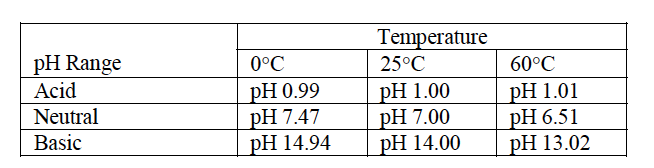
\includegraphics{/Users/abhisreekanth/Desktop/ChemHL-IA/Figures/1.png}
	\caption{Relationship of pH and temperature (Ashton and Geary, 2005).}
\end{figure} 
\noindent
The pH of a solution varies with concentration as well. There is a linear relationship between the concentration of a solution and its subsequent pH. This is because the pH of a solution is the measure of the hydrogen ion concentration of the solution. For every increase in pH by a factor of 1, the concentration increases by a factor of ten. \\
\noindent
%pKa & 
The acid dissociation constant, $K_a$, is the measure of the strength of an acid in solution. The $K_a$ is found by solving the expression for the following acid dissocation reaction: \\

\begin{eqnarray*}
\ce{ HA_{\aq} <=> H^{+}_{\aq} + A^{-}_{\aq} }
\end{eqnarray*}

\noindent
Where HA is the generic acid, $H^+$ is the hydrogen ion, and $A^-$ is the conjugate base of the acid. The above reaction is in equilibrium when the concentrations of all the elements in the reaction is constant. The acid dissocation constant is therefore the products over the reactants as shown below:

\begin{eqnarray*}
K_a = \frac{[H^+][A^-]}{HA}
\end{eqnarray*} \\

\noindent
From the acid dissociation constant, the $pK_a$T of the acid can be derived. The $pK_a$ of an acid states the acidity of a given hydrogen atom of excatly one molecule of that acid. The $pK_a$ of an acid is essentially the pH at which it is exactly half dissociated. The $pK_a$ of the acid can be mathematically calculated as the negative logarithm of the acid dissociation constant, as shown in the equation below. 
\begin{eqnarray*}
pK_a = -\log_{10}K_a
\end{eqnarray*} \\

\noindent
The larger the value of the $pK_a$, the lesser the dissociation of the acid, thereby indicating a weak acid. The smaller the value of the $K_a$, the weaker the acid. Therefore, the smaller the value of the $pK_a$, the greater the dissociation of the acid, indicating a strong acid. The larger the value of the $K_a$ the stronger the acid. \\\\
%buffers
\noindent
A buffer solution is a solution which consists of a weak Bronsted acid and its conjugate base, or a weak Bronsted base and its conjugate acid. Buffer solutions are quite resistant to pH changes, when small quantities of acid are added, as well. \\\\
\noindent
There are two types of buffer solutions: Acidic and Alkaline. Acidic buffer solutions have a pH less than 7, and are composed of weak acids and its conjugate base. Alkaline buffer solutions have a pH greater than 7, and are composed of weak bases and its conjugate acid. \\\\
\noindent
Buffer solutions essentially work by removing any hydrogen or hydroxide ions which might be added to it, thereby not changing the pH of the solution when an acid or base is added to it. \\\\
\noindent
Buffer solutions are paramount to industry due to the inumerable practical applications which are present. One such industry is pharmaceuticals. in the Pharmaceutical industry, many therapeutic drugs are synthesizied to form buffer solutions to increase the shelf-life of the drugs, ensure the stability of treatments,  maintaing the drug at a near neutral, constant pH to avoid irratition with skin, and much more. 
Buffer solutions are used in fermentation reactions, such as beer and yogurt, to ensure that there are no harsh changes and to achieve maximum yield. Buffers are also used in the manufacture of glue to ensure that there aren't changes in the highly sensitive chemical gelatine. Lastly, buffers are used in the soap industry to create soap with a pH of 5.5, the pH of our skin, and to avoid any irritation with our skin. \\\\
\noindent
%previous study  
In a study conducted by Gerardo Gomez, Michael J. Pikal, and Nair Rodriguez-Hornedo, the pH changes of buffers were measured when Sodium Phospate buffers were induced by Salt percipitation during various far-from-equilibrium freezing temperatures. It was concluded that the greatest variations in pH occured at lower freezing temperatures around $-10^o C$. There was a linear correlation between colder temperatures and greater variations, as the temperature was closer to $-10^o C$, the greater the variation in pH from the buffer's initial equilibrium value. \\\\
\noindent
This begged the question: How would the pH of a buffer soultion vary with an increase in temperature. This study was not only conducted to answer that very question, but also conducted to explore the practical implications involved with understanding the relationships of buffers and its subsequent pH. After determining the pH the effects on the $K_a$ of the acid can be explored, thereby determining how an increase in the temperature of a buffer can affect the stregth of an acid. This knowledge can help various companies determine the proper temperature in which their buffers must be created, thereby maximizing profit, time, and the accuracy of the pH of the buffer.  
\subsection*{Hypothesis}%Hypothesis
If an increase in the temperature of an Acid increases its pH; thereby increasing the decreasing the strength of the acid, then an increase temperature of the buffer solution between Acetic Acid, \ce{C_2H_4O_2}, and Sodium Acetate, \ce{C_2H_3NaO_2}, will cause an increase in temperature; thereby, weakening the acid. 
\subsection*{Safety Information}%Safety Information
Safety is paramount, and good laboratory practices should not only be informed, but also practiced. The risk of burn was apparent, all throughout the experiment. Simple measures must be taken to prevent any sort of burn injuries. The hot-plates used, and hot beakers should be stationed at an area, away from foot traffic. Proper equipment should be used to touch and move the hot equipment, and lastly, safety googles must be worn at all times, in case of splattering.
\section*{Materials} %Materials
%Use Enumerate Here 
\begin{enumerate}
\item Acetic Acid (50 mL)
\item Sodium Acetate (15 g)
\item 50 mL Beaker (3)
\item 150 mL Beaker (1)
\item pH Probe (1)
\item Temperature Probe (1)
\item Hot Plate (1)
\end{enumerate}
\section*{Methods}%Methods

\section*{Procedure} %Procedure

\section*{Results} %Results
\subsection*{Raw Data} %Raw Data

\subsection*{Calculations}%Calculations

\section*{Discussion}%Discussion
\subsection*{Conclusion}

\subsection*{Experimental Error} %Experimental Error 

\subsection*{Improvements} %Improvements 

\end{document}